\documentclass[a4paper,twoside,DIV15,BCOR12mm]{scrbook}

%exam will consist of 2-4 excercises, 1h wiht 60 points meaning 1min for 1 point
%per exercie there a 2 - 4 part
%discuss paper, extend design, how to improve, report main questions, main designs, etc.

\usepackage{Econ}

%standard setup
\author{Prof. Dr. Nora Szech}
\publishers{Martin Belica}
\title{Economics and Behaviour}
\date{Wintersemester 2015}

%latexki
\author{Prof. Dr. Nora Szech}
\semester{Wintersemester 2015}
\scriptstate{work-in-progress}

\makeindex

\begin{document}

\pagenumbering{arabic}
\setcounter{page}{1}

%!TEX root = Funktionalanalysis - Vorlesung.tex

\maketitle
%!TEX root = Funktionalanalysis - Vorlesung.tex

%\chapter*{Vorwort}
%Dieses Skript wurde im Wintersemester 2015/2016
%von Martin Belica geschrieben. Es beinhaltet die Mitschriften aus
%der Vorlesung von Prof.~Dr.~Szech sowie die Mitschriften einiger
%Übungen.


\chapter*{Content of teaching}

The course covers topics from behavioral economics with regard to contents and methods. In addition, the students gain insight into the design of economic experiments. Furthermore, the students will become acquainted with reading and critically evaluating current research papers in the field of behavioral economics. \\
  
\textbf{Prerequisites} \\
None. Recommendations: Basic knowledge of microeconomics and statistics are recommended. A background in game theory is helpful, but not absolutely necessary. \\

\textbf{Aim} \\
The students gain insight into fundamental topics in behavioral economics;
get to know different research methods in the field of behavioral economics;
learn to critically evaluate experimental designs;
get introduced to current research papers in behavioral economics;
become acquainted with the technical terminology in English. \\

\textbf{Bibliography} \\
\begin{itemize}
	\item Kahnemann, Daniel: Thinking, Fast and Slow. Farrar, Straus and Giroux, 2011.
	\item Ariely, Dan: Predictably irrational. New York: Harper Collins, 2008.
	\item Ariely, Dan: The Upside of Irrationality. New York: HarperCollins, 2011. 
\end{itemize}	

\tableofcontents

%!TEX root = Economics and Behaviour.tex


\chapter{Standard theoretic basics for analysis of strategic behaviour}

First, a strategic interaction occurs when the utility of actors, e.g. players (individuals, companies, ...) in a situation is mutually influenced by individual behavioural changes. 

A \begriff{game} is a formal representation of a situation in which a number of individuals interact in a setting of \textit{strategic interdependence}.
	We have to clarify four points:
	\begin{itemize}
		\item The players: Who is interacting?
		\item When do they move or what can they do?
		\item The outcomes: For each possible set of actions by the players, what is the outcome of the game?
		\item The payoffs: What are the players' preferences over the possible outcomes?
	\end{itemize}

For example Tick-Tack-Toe games, auctions or even meetings can be described with games. 

\index{equilibrium} % todo definituon
In the following two sections equilibria are one of our main focus point. Three properties describe such a state, where economic forces are balanced and in the absence of external influences the behaviour leading to the equilibrium will not change:
\begin{enumerate}
	\item The behaviour of agents in such a point is consistent.
	\item No agent has an incentive to change its behaviour.
	\item The equilibrium is the outcome of some dynamic process (stability).
\end{enumerate}

~\newline
Subsequent, we distinguish between the formal representation which we use to model the conflict situation, however all situations we will examine will have complete information.

\newpage
%!TEX root = Economics and Behaviour.tex


\chapter{Standard theoretic basics for analysis of strategic behaviour}


\section{Games in strategic form}
For two players ($P1$ and $P2$) and two possible signals (lets call them $a$ and $b$) we usually use the matrix form to display a game, where $u_{i}(x, y)$ represents the utility function for player $i$ given the signal $x$ for $P1$ and the signal $y$ for $P2$ with $x, y \in \{ a, b\}$
\begin{center}
	\begin{tabular}{|c|c|c|}
		\hline\hline
  			$P1$ / $P2$ & \textbf{a} & \textbf{b} \\
         		\cline{1-3}
   					\textbf{a} & $( u_{1}(a, a) , u_{2}(a, a))$ & $(u_{1}(a, b), u_{2}(a, b))$	\arrayrulewidth2pt \\
            	\cline{1-3}
   					\textbf{b} & $( u_{1}(b, a), u_{2}(b, a))$ & $(u_{1}(b, b), u_{2}(b, b))$\\ \hline\hline
	\end{tabular}	
\end{center}

We call a \begriff{set of strategies} complete plan of actions for each situation in a game.

\begin{example}[Prisoner's Dilemma] \label{prisonersdilemma} \index{Prisoner's Dilemma}
	 Image, two members of a criminal gang are arrested and imprisoned. Each prisoner is in solitary confinement with no means of communicating with the other. The prosecutors lack sufficient evidence to convict the pair on the principal charge. They hope to get both sentenced to a year in prison on a lesser charge. Simultaneously, the prosecutors offer each prisoner a bargain. Each prisoner is given the opportunity either to: betray the other by testifying that the other committed the crime, or to cooperate with the other by remaining silent. The offer is:
	\begin{itemize}
		\item If A and B each betray the other, each of them serves 6 years in prison
		\item If A betrays B but B remains silent, A will be set free and B will serve 9 years in prison (and vice versa)
		\item If A and B both remain silent, both of them will only serve 1 year in prison (on the lesser charge)
	\end{itemize}
	
\begin{center}
	\begin{tabular}{|l|l|r|}
		\hline\hline
  			P1 / P2 & \textbf{defects} & \textbf{cooperates} \\
         		\cline{1-3}
   			\textbf{defects} & $(-6, -6)$ & $(0, -9)$ 	\arrayrulewidth2pt \\
            	\cline{1-3}
   			\textbf{cooperates} & $(-9, 0)$ & $(-1, -1)$ \\ \hline\hline
	\end{tabular}	
\end{center}


	Other Interpretations of the Prisoner's Dilemma
	\begin{itemize}
		\item Collusion on prices
		\item Investing in human capital vs. arming for a war
		\item Buying a SUV vs. a smaller car
	\end{itemize}
\end{example}


\subsection{Dominant strategies}

\begin{definition}[Strict dominance] \index{strictly dominated}
	A strategy $s_{i}''$ is strictly dominated if and only if there exists another strategy $s_{i}'$ such that
	\[ u(s_{i}', s_{-i}) \geq u(s_{i}'', s_{-i}) \quad \forall s_{-i} \in S_{i} \]	
\end{definition}

In the \hyperref[prisonersdilemma]{Prisoner's Dilemma} $cooperate$ is strictly dominated by $defect$. Simply the elimination of strictly dominated strategies leads to the prediction of $(defects, defects)$, even though $(cooperates, cooperates)$ would result in a lower prison sentence.


\begin{example}
	Iterated elimination of strictly dominated strategies leads to
	\begin{itemize}
		\item for Player 2: $l$ strictly dominates $r$
		\item after having eliminated $r$ we can further eliminate $d$, since $d$ is then strictly dominated by $u$
	\end{itemize}
\end{example}

Important to notice is that here, the prediction we derived relies immensely on the rationality of all players.

\begin{definition}[Weak dominance] \index{weakly dominated}
	A strategy $s_{i}''$ is weakly dominated by $s_{i}'$ if and only if for all possible outcomes 
	\[ u(s_{i}', s_{-i}) \geq u(s_{i}'', s_{-i}) \quad \forall s_{-i} \in S_{i} \]	
	and there exists at least one outcome where
		\[ u(s_{i}', s_{-i}) > u(s_{i}'', s_{-i}) \quad \forall s_{-i} \in S_{i} \]	 
\end{definition}

\subsection{Nash-Equilibrium}

\begin{definition}[A strategy profile] \label{strategyprofile} \index{strategy profile}
	We call a vector $S = (S_{1}, \dotsc, S_{N})$ of dimension $N$ that specifies a strategy for every player in the game a strategy profile.
\end{definition}

\begin{definition}[Nash-Equilibrium] \label{nashequilibrium} \index{Nash-Equilibrium}
	An informal definition of a Nash-Equilibrium would be that it is the mutual best response for every player, therefore a strategy profile in which no player can do better by unilaterally changing their strategy. \\
	Defining it formally would mean: a strategy profile $x^{*} \in S$ is a Nash-Equilibrium if no unilateral deviation in strategy by any single player is profitable for tat player, that is
	\[ \forall i \in \{1, \dotsc, N \},~ x_{i} \in S_{i} : \quad u_{i}(x_{i}^{*}, x_{-i}^{*}) \geq u_{i}(x_{i}, x_{-i}^{*}) \]
	\end{definition}

\begin{example}[Battle of the sexes] \label{battleofthesexes} \index{Battle of sexes}
		The next example is a two-player coordination game. \\
		Image a couple that agreed to meet this evening, but both individually cannot recall if they will be attending the opera or a football match. The husband would most of all like to go to the football game. The wife would like to go to the opera. Both would prefer to go to the same place rather than different ones. \\ \\
		Hence, the Battle of sexes in strategic form could look something like:
		
		\begin{center}
			\begin{tabular}{|l|l|r|}
				\hline\hline
  					M / F & \textbf{football} & \textbf{opera} \\
         				\cline{1-3}
   					\textbf{football} & $(1, 2)$ & $(0, 0)$ 	\arrayrulewidth2pt \\
            			\cline{1-3}
   					\textbf{opera} & $(0, 0)$ & $(2, 1)$ \\ \hline\hline
			\end{tabular}	
		\end{center}
		2
		The two Nash-Equilibriums in this game are $(opera, opera)$ and $(football, football)$ since
		\[ u_{i}(opera, opera) \geq u_{i}(football, opera) \quad \forall i \in \{ 1, 2 \} \]
\end{example}

\begin{example}[The Beauty-Contest] \index{Beauty-Contest}
Keynes described the action of rational agents in a market using an analogy based on a fictional newspaper contest, in which entrants are asked to choose the six most attractive faces from a hundred photographs. Those who picked the most popular faces are then eligible for a prize. The agents has to consider that not his preferred choice is the optimal strategy but the one with the highest chances to be chosen by all others. \\

	The rest is missing in my notes. %todo: missing in my notes
\end{example}

\subsection{Sub-game-Perfect Nash-Equilibrium}


\begin{example}[Dictator-Game] \index{Dictator-Game}
Proposer $P$ can split up 10 \euro ~ (up to \euro-level) between him and a Receiver $R$. 
	\begin{itemize}
		\item Question 1: Assume for a minute the Proposer $P$ is totally selfish and only cares about his own profits. Is there a strictly dominant strategy for $P$? \\
			Yes! $(10, 0)$ (money Proposer, money Receiver) is strictly dominant.
		\item Question 2: What if $P$ is a pure altruist and just cares about the money $R$ gets? \\
			Then $(0, 10)$ is strictly dominant.
	\end{itemize}
\end{example}


The Dictator-Game is nicely analysed by Christoph Engel in his book \textit{Dictator-Games: A meta study (2011)}. In the following part we'd like to look at a modification of the Dictator-Game:

\begin{example}[Ultimatum-Game]	\label{ultimatumgame} \index{Ultimatum-Game} 
The Ultimatum-Game is a dynamic game under complete information. \\
We look at two players in two stages. The first player (the proposer (P)) receives a sum of money $(M = 10)$ and proposes how to divide the sum between himself $(x_{p})$, where $x_{p} \in \{ 0, 1, 2, \dotsc, 10 \}$, and another player $(10 - x_{p})$. The second player (the responder (R)) chooses to either accept or reject this proposal. If the second player accepts, the money is split according to the proposal. If the second player reject, neither player receives any money.

Lets sum this up again:
	\begin{itemize}
		\item P proposes split up $(x_{p}, 10 - x_{p})$
		\item R accepts or rejects
			\begin{itemize}
				\item If R accepts $(a)$, proposal becomes implemented. P receives $x_{p}$ and R $10 - x_{p}$
				\item If R rejects $(r)$, the whole money gets destroyed.
			\end{itemize}
	\end{itemize}
	
	\begin{center}
		\begin{tikzpicture}[auto, level distance=30mm, sibling distance=35mm]
			\node [circle,draw] (z){$P$}
 						child {node [circle,draw] (a) {$10$}	}
 						child {node [] (b) {$ $}	}
 						child {node [circle,draw] (c) {$x_{p}$}
  							child {node [circle,draw] (f) {$(x_{p}, 10 - x_{p})$}	}
  			 				child {node [circle,draw] (g) {$(0, 0)$}	}			
 						}
 						child {node [] (d) {$$}	}
  						child {node [circle,draw] (e) {$0$}
			};
			\path (a) -- (b) node [midway] {$\dotsc$};
			\path (b) -- (c) node [midway] {$\dotsc$};
			\path (c) -- (d) node [midway] {$\dotsc$};
			\path (d) -- (e) node [midway] {$\dotsc$};
			\path (f) -- (g) node [midway] {$a$ $/$ $r$};
		\end{tikzpicture}				
	\end{center}
	
	A strategy set in this game would have to look like
	\begin{itemize}
		\item Proposer sets a $x_{p}$
		\item Receiver decides for \textit{any} $x_{p}$ that might come up if he'd accept or reject that offer.
	\end{itemize}
	\begin{center}( a strategy needs to specify a complete action plan. ) \end{center}
	
	
	\textbf{1. Question:} Can the outcome $(5, 5)$ be stabilised as a Nash-Equilibrium? \\
	\textbf{Answer:} Yes. Say P proposes $x_{p} = 5$ and the strategy set for R is defined by accepting for any value of $x_{p} \leq 5$ and rejecting the offer for values larger than $5$. \\
		In this situation $(5, 5)$ would be stabilised as a Nash-Equilibrium.


	\textbf{2. Question:} Is there another Nash-Equilibrium that stabilises the $(5, 5)$ outcome? \\
	\textbf{Answer:} Yes. If P again proposes $x_{p} = 5$ and the strategy set for R is defined by accepting for only $x_{p} = 5$ and rejecting for any other case, so $x_{p} \neq 5$. 
	
	
	\textbf{3. Question:} Can $(0, 10)$ be stabilised as a Nash-Equilibrium? \\
	\textbf{Answer:} Yes. We set the strategy for P as $x_{p} = 0$ and for R demand accepting for $x_{p} = 0$ and rejecting for any other case, meaning for $x_{p} \geq 1$. 
\end{example}

As we can see the Nash-Equilibrium can lead to an infinite amount of outcomes some of them even with implausible threats. We'd therefore like to refine this kind of equilibrium which leads us to the (sub-game) perfect Nash-Equilibrium.

\begin{definition}[Sub-game] \index{sub-game}
	A sub-game is any part of a game that meets the following criteria:
	\begin{itemize}
		\item It has a single initial node that is the only member of that node's information set (i.e. the initial node is in a singleton information set).
		\item If a node is contained in the sub-game then so are all of its successors
		\item If a node in a particular information set is in the sub-game then all members of that information set belong to the sub-game.
		\item and finally the node must not contain a deterministic state but instead at least one non-trivial choice
	\end{itemize}
\end{definition}

\begin{definition}[(Sub-game-)Perfect Nash-Equilibrium] \index{Sub-game-Perfect Nash-Equilibrium} 
A strategy profile is a Sub-game-Perfect Nash-Equilibrium if it represents a Nash equilibrium of every sub-game of the original game. Informally, this means that if the players played any smaller game that consisted of only one part of the larger game and their behaviour represents a Nash equilibrium of that smaller game, then their behaviour is a sub-game perfect equilibrium of the larger game. 

	How to find a Perfect Nash-Equilibrium:
	\begin{enumerate}
		\item Define (one set of) optimal actions for the last sub-game
		\item Replace that decision nodes with the respective outcome
		\item Repeat $(1)$ and $(2)$ until the first decision node.
	\end{enumerate}
\end{definition}

\begin{example}[Sequel to the Ultimatum-Game]
	Searching for the Perfect Nash-Equilibrium in this case leads to:
	\begin{enumerate}
		\item Defining the optimal actions
			\begin{itemize}
				\item In the case $P$ chooses $x_{p} = 10$, then $R$ receives  $10 - x_{p} = 0$ and he is 	indifferent between refusing and accepting. Let's assume for now he'd accept in this case.
				\item In all other cases, meaning $x_{p} \in [0, 10)$, would R receive $10 - x_{p} > 0$. Therefore he would accept the offer in all cases.
			\end{itemize}
		\item Now we can reduce the game to the following game tree
			\begin{center}
				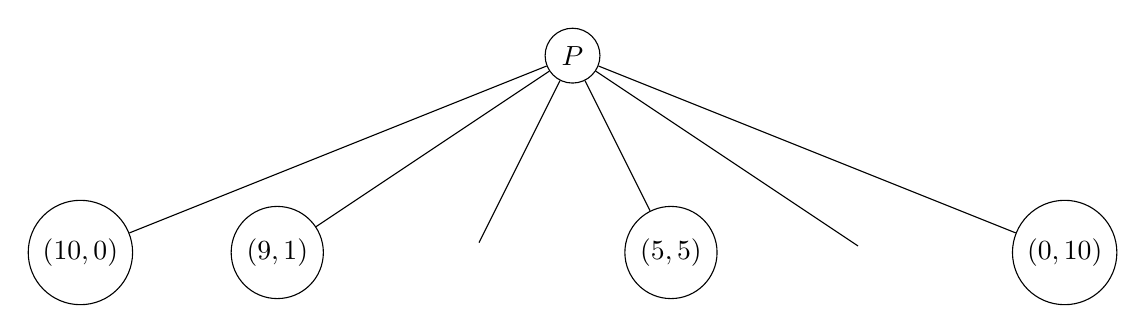
\begin{tikzpicture}[level/.style={sibling distance=25mm/#1}, level 	distance=25mm]
					\node [circle,draw] (z){$P$}
 						child {node [circle,draw] (a) {$(10, 0)$}	}
 						child {node [circle,draw] (b) {$(9, 1)$}	}
 						child {node [] (c) {$ $}	}
 						child {node [circle,draw] (d) {$(5, 5)$}	}
 						child {node [] (e) {$ $}	}
  						child {node [circle,draw] (f) {$(0, 10)$}
					};
					\path (b) -- (c) node [midway] {$\dotsc$};
					\path (c) -- (d) node [midway] {$\dotsc$};
					\path (d) -- (e) node [midway] {$\dotsc$};
					\path (e) -- (f) node [midway] {$\dotsc$};
				\end{tikzpicture}				
			\end{center}
		\item Since we have already reached the first node, a simple analyse of the reduced situation for Nash-Equilibriums returns the Sub-Game-Perfect Nash-Equilibrium. In this situation $P$ is supposed to chose $x_{p} = 10$ since it results in the highest utility value.
	\end{enumerate}
	$\Rightarrow P$ playing $x_{p} = 10$ together with R always accepting constitutes a Sub-game-Perfect Nash-Equilibrium. 

	If we look for another equilibrium it yields
		\begin{enumerate}
		\item the optimal actions
			\begin{itemize}
				\item Again, in all cases $x_{p} \in [0, 10)$ would R receive $10 - x_{p} > 0$, therefore he'd accept the offer in all cases.
				\item If he now would refuse to the offer $x_{p} = 10$ it would be plausible therefore sub-game perfect, since he indifferent between both choices.
			\end{itemize}
		\item the tree changes only slightly:
			\begin{center}
				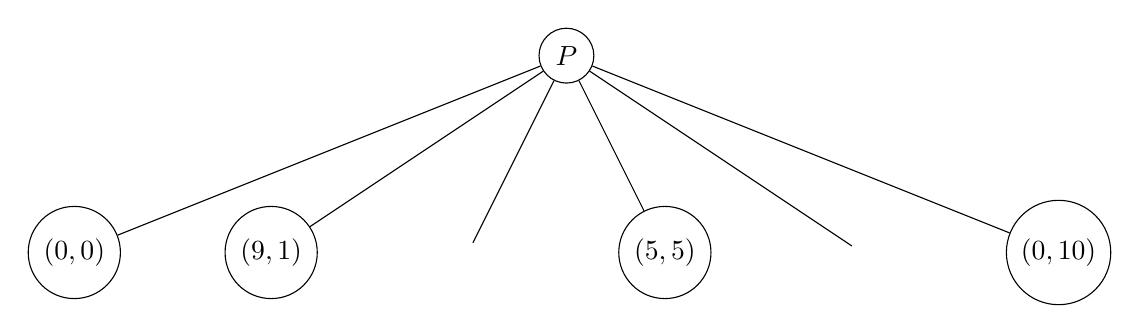
\begin{tikzpicture}[level/.style={sibling distance=25mm/#1}, level 	distance=25mm]
					\node [circle,draw] (z){$P$}
 						child {node [circle,draw] (a) {$(0, 0)$}	}
 						child {node [circle,draw] (b) {$(9, 1)$}	}
 						child {node [] (c) {$ $}	}
 						child {node [circle,draw] (d) {$(5, 5)$}	}
 						child {node [] (e) {$ $}	}
  						child {node [circle,draw] (f) {$(0, 10)$}
					};
					\path (b) -- (c) node [midway] {$\dotsc$};
					\path (c) -- (d) node [midway] {$\dotsc$};
					\path (d) -- (e) node [midway] {$\dotsc$};
					\path (e) -- (f) node [midway] {$\dotsc$};
				\end{tikzpicture}				
			\end{center}
	\end{enumerate}
	$\Rightarrow P$ playing $x_{p} = 9$ together with R always accepting if $x_{p} < 10$ and refuses for $x_{p} = 10$ also constitutes a Sub-game-Perfect Nash-Equilibrium. 
\end{example}


\begin{example}[Guessing-Game / Beauty-Contest] \index{Guessing-Game}
	In a game with at least two players we can describe the sequel for the Guessing-Game as following
	\begin{itemize}
		\item $n \geq 2$ players
		\item Every player guesses a number $b_{i} \in \{0, 1, 2, \dotsc, 100 \}$
		\item Goal is to guess $b_{i}$ as close as possible to $\frac{p}{n} \cdot \sum_{i = 1}^{n} b_{i} = p \cdot \varnothing, \quad p \in (0, 1)$
		\item The best guess (closes to $p \cdot \varnothing$) wins, in case of a tie a random device that is 'fair' decides who win the price $P > 0$
	\end{itemize}
	
	
	\textbf{1. Question:} Is $(0, \dotsc, 0)$ a Nash-Equilibrium? \\
	\textbf{Answer:} Yes. Assume all bidders except for bidder $i$ bid $0$.	
		\begin{itemize}
			\item if bidder $i$ bids $0$ expected win equals $\frac{1}{n} P $
			\item if bidder $i$ bids something above $0$ his expected profit is going to be $0$ as $0$ is closer to $p \cdot \varnothing$ then the bet $b > 0$ of player $i$:
			\[ p \cdot \varnothing = p \frac{(n - 1)0 + 1 b}{n} = p \frac{b}{n} \]
			\[
				d \left( b, p \frac{b}{n} \right) > d \left( p \frac{b}{n}, 0 \right)	\gdw \left| b - p \frac{b}{n} \right| > \left| p \frac{b}{n} \right| \quad
			\]
			
			and since $b > p \cdot \varnothing$ we can simplify this further to
			\[ b > \left( p \cdot b \right) \cdot \frac{2}{n} \quad \text{and this holds since } n \geq 2 \text{ and } p < 1.\]
		\end{itemize}
		
	
	\textbf{2. Question:} is $(0, \dotsc, 0)$ the unique Nash-Equilibrium here? \\
	\textbf{Answer:} Yes, since:	
	\[ b_{i}^{*} \leq \frac{1}{2} \frac{\sum_{j \neq i} b_{j}^{*}}{n - 1} \]
	\begin{align*}
		\Rightarrow \sum_{i = 1}^{n} b_{i}^{*} \leq \frac{1}{2} \frac{\sum_{i = 1}^{n} \sum_{j \neq i} b_{j}^{*}}{n - 1} & = \frac{1}{2} \frac{(n - 1) \sum_{j = 1}^{n} b_{j}^{*}}{n - 1} \\
		& = \frac{1}{2} \sum_{j = 1}^{n} b_{j}^{*}
	\end{align*} 
	\[ \gdw \sum_{i = 1}^{n} b_{i}^{*} \leq \frac{1}{2} \sum_{i = 1}^{n} b_{i}^{*} \]
	therefore only $(0, \dotsc,  0)$ can be a Nash-Equilibrium in this situation. \\


	\textbf{3. Question:} is $(0, \dotsc, 0)$ also a strictly dominant strategy? \\
	\textbf{Answer:} No. By analysing the following situation we find a counterexample: \\
	$50$ players. $48$ of them bid the number $100$, bidder $49$ bids $0$ then the optimal strategy for player $50$ is to bid $97$. \\
	Therefore $0$ is not the best answer and cannot be a strictly dominant strategy.
\end{example}


\newpage
%!TEX root = Economics and Behaviour.tex


\chapter{An ultimatum game with multidimensional response strategies} 

\section{Presented papers}


\begin{itemize}
	\item Güth, W.; Levati, M.V.; Nardi, C.; Soraperra, I. (2014): An ultimatum game with multidimensional response strategies. In Jena Economic Research Papers, FriedrichSchiller University and Max Planck Institute of Economics, Jena, Germany (Ultimatum Game)
		\begin{itemize}
			\item \textbf{An ultimatum game with multidimensional response strategies} \\
			Negotiations frequently end in conflict after one party rejects a final offer. In a large-scale Internet experiment, we investigate whether a 24-hour cooling-off period leads to fewer rejections in ultimatum bargaining. We conduct a standard cash treatment and a lottery treatment, where subjects receive lottery tickets for several large prizes. In the lottery treatment, unfair offers are less frequently rejected, and cooling off reduces the rejection rate further. In the cash treatment, rejections are more frequent and remain so after cooling off. We also study the effect of subjects’ degree of “cognitive reflection” on their behaviour.
		\end{itemize}
\end{itemize}


\newpage
%!TEX root = Economics and Behaviour.tex


\chapter{Cooling Off in Negotiations: Does It Work?}

\section{Presented papers}

\begin{itemize}
	\item Oechssler, J.; Roider, A.; Schmitz, P. (2015): Cooling Off in Negotiations: Does it Work?. Journal of Institutional and Theoretical Economics JITE J Inst Theor Econ 171, (2015). (Ultimatum Game)
\end{itemize}



\newpage
%!TEX root = Economics and Behaviour.tex

\section{Level k as a prominent example of a nonstandard/behavioural approach}


\textbf{Unraveling in Guessing Games: An Experimental Study}

\begin{itemize}
	\item Nagel, R. (1995): \textit{Unraveling in Guessing Games: An Experimental Study}. In: American Economic Review.
		\begin{itemize}
			\item Consider the following game: a large number of players have to state in several rounds simultaneously a number in the closed interval [0, 100]. The winner is the person whose chosen number is closest to the mean of all chosen numbers multiplied by a parameter $p$, where $p$ is common knowledge. The payoff to the winner is a fixed amount, which is independent of the stated number and $p$. If there is a tie, the prize is divided equally among the winners. The other players whose chosen numbers are further away receive nothing.
		\end{itemize}
\end{itemize}	
			
\textbf{More than Meets the Eye}

\begin{itemize}
	\item Müller, J.; Schwieren, C. (2011): \textit{More than Meets the Eye: an Eye-tracking Experiment on the Beauty Contest Game}
		\begin{itemize}
			\item The beauty contest game has been used to analyse how many steps of reasoning subjects are able to perform. A common finding is that a majority seem to have low levels of reasoning. We use eye-tracking to investigate not only the number chosen in the game, but also the strategies in use and the numbers contemplated. We can show that not all cases that are seemingly level-1 or level-2 thinking indeed are – they might be highly sophisticated adaptations to beliefs about other people’s limited reasoning abilities.
		\end{itemize}
\end{itemize}		

\newpage
%!TEX root = Economics and Behaviour.tex


\chapter{Organizations and Markets: The role of market incentives}

\section{Presented papers}

\begin{itemize}
	\item Gneezy, U.; Rustichini, A. (2000): \textit{Pay Enough or Don't Pay at All}. In: Quarterly Journal of Economics.
	\item Gneezy, U.; Rustichini, A. (2000): \textit{A Fine is a Prise}. In: The Journal of Legal Studies. (monetary incentives)
	\item Sebastian Kube, Michel Andre Marechal and Clemens Puppe (2012): \textit{The Currency or Reciprocity: Gift Exchange in the Workplace}. In: American Economics Revie. (money versus non-monetary incentives)
	\item Charness, G.; Grieco, D. (2014): \textit{Creativity and Financial Incentives} 
\end{itemize}


\newpage
%!TEX root = Economics and Behaviour.tex

\chapter{Organisations and Markets: The role of moral dimensions of markets}

\section{Morals and Markets}
\section{You Owe Me}
\section{How Customers' insurance coverage induces sellers' misbehaviour}

\begin{itemize}
	\item Falk, A.; Szech, N. (2013): \textit{Morals and Markets}. In: Science (moral dimensions)
		\begin{itemize}
			\item The possibility that market interaction may erode moral values is a long-standing, but controversial, hypothesis in the social sciences, ethics, and philosophy. To date, empirical evidence on decay of moral values through market interaction has been scarce. We present controlled experimental evidence on how market interaction changes how human subjects value harm and damage done to third parties. In the experiment, subjects decide between either saving the life of a mouse or receiving money. We compare individual decisions to those made in a bilateral and a multilateral market. In both markets, the willingness to kill the mouse is substantially higher than in individual decisions. Furthermore, in the multilateral market, prices for life deteriorate tremendously. In contrast, for morally neutral consumption choices, differences between institutions are small.
		\end{itemize}
	\item Malmendier, U.; Schmidt, K. (2012): \textit{You Owe Me}. In: DOI (moral dimensions)
		\begin{itemize}
			\item In many cultures and industries gifts are given in order to influence the recipient, often at the expense of a third party. Examples include business gifts of firms and lobbyists. In a series of experiments, we show that, even without incentive or informational effects, small gifts strongly influence the recipient’s behaviour in favour of the gift giver, in particular when a third party bears the cost. Subjects are well aware that the gift is given to influence their behaviour but reciprocate nevertheless. Withholding the gift triggers a strong negative response. These findings are inconsistent with the most prominent models of social preferences. We propose an extension of existing theories to capture the observed behaviour by endogenising the “reference group” to whom social preferences are applied. We also show that disclosure and size limits are not effective in reducing the effect of gifts, consistent with our model. Financial incentives ameliorate the effect of the gift but backfire when available but not provided.
		\end{itemize}
	\item Kerschbamer, R.; Neururer, D.; Sutter, M. (2014): \textit{How Customers' insurance coverage induces sellers' misbehaviour in markets for credence goods}
		\begin{itemize}
			\item Markets for credence goods are characterised by informational asymmetries between expert sellers and their customers, which creates strong incentives for fraudulent behaviour of sellers that results in estimated annual costs to customers and the society as a whole of billions of dollars in the US alone. Prime examples of credence goods are all kinds of repair services, the provision of medical treatments, the sale of software programs, and the provision of taxi rides in unfamiliar cities. In this paper, we examine in a natural field experiment how insurance coverage on the side of the consumer – often prevalent on important markets such as the health care or repair services sectors – can seriously exacerbate inefficiencies in the provision of credence goods by inducing misbehaviour on the side of the seller. Specifically, we study how computer repair shops take advantage of customers’ insurance for repair costs. In a control treatment, the average repair price is about Euro 70, with the repair bill increasing to Euro 129 when the service provider is informed that the insurance would reimburse the bill. Our design allows for a decomposing of the sources of this economically impressive and statistically highly significant difference showing that this is mainly due to the over-provision of parts and overcharging of working time. Overall, our results strongly suggest that insurance coverage greatly increases the extent of misbehaviour of sellers in important sectors of the economy with potentially huge costs to customers and whole economies.
		\end{itemize}
\end{itemize}

\newpage
%!TEX root = Economics and Behaviour.tex


\chapter{Ethics in science}

\section{Pleasures of Skill and Moral Conduct}
Background:
\begin{itemize}
	\item Jeremy Bentham pointed fourteen different $"$simple$"$ sources of pleasures for humans out
	\item In this short list, number three is the $"$pleasure of skill$"$ while number five is $"$the pleasure of a good name$"$.
	\item Yet if being skilful is of crucial importance to people than this can oppose the possibility to keep a good name
\end{itemize}
  
  
  
\textbf{As an example: The Manhattan Project.} After the dropping of the plutonium bomb on Nagasaki, numerous members of the Manhattan Project started worrying about moral implications. Many of the scientists suffered from e.g depressions. \\ 

The Self-Image is so relevant in this concept. Both the desire for mastery and acting in accordance with moral values originate from the same source, a desire for positive self-image. \\ 

The remaining question is therefore: does morality in some (everyday) situations get traded off against skilfulness?

\begin{itemize}
	\item Falk, A.; Szech, N. (2016): \textit{Pleasures of Skill and Moral Conduct}. KIT working paper. (non-monetary incentives and morals)
		\begin{itemize}
			\item As was recognised by Bentham, skilfulness is an important source of pleasure. Humans like achievement and to excel in tasks relevant to them. This paper provides controlled experimental evidence that striving for pleasures of skill can have negative moral consequences and causally reduce moral values. In the study, subjects perform an IQ-test. They know that each correctly solved question not only increases test performance but also the likelihood of moral transgression. In terms of self-image, this creates a trade-off between signalling excellence and immoral disposition. We contrast performance in the IQ-test to test scores in an otherwise identical test, which is, however, framed as a simple questionnaire with arguably lower self-relevance. We find that subjects perform significantly better in the IQ-test condition, and thus become more willing to support morally problematic consequences. Willingness to reduce test performance in order to behave more morally is significantly less pronounced in the IQ versus the more neutral context. The findings provide controlled and causal evidence that the desire to succeed in a challenging, self-relevant task has the potential to seduce subjects into immoral behaviours and to significantly decrease values attached to moral outcomes.
		\end{itemize}
\end{itemize}


\section{The Social Responsibilities of Scientists}

\begin{itemize}
	\item Russell, B. (1960): \textit{The Social Responsibilities of Scientists}. In: Science, New Series.
		\begin{itemize}
			\item A scientist can no longer shirk responsibility for the use society makes of his discoveries.
		\end{itemize}
\end{itemize}


\section{The Moral UnNeutrality of Science}

\begin{itemize}
	\item William 0. Baker and more (1961): \textit{The Moral UnNeutrality of Science}: The scientist's special responsibility are examined an address given at the 1960 AAAS annual meeting. In: Science.
		\begin{itemize}
			\item The scientist's special responsibilities are examined in an address given at the 1960 AAAS annual meeting
		\end{itemize}
\end{itemize}


\newpage
%!TEX root = Economics and Behaviour.tex

\chapter{Non-standard utility}


\section{Anticipatory utility}

The standard utility approach would state an already deterministic situation and it's utility for an individual is not changed by additional information. Nevertheless:

\begin{itemize}
	\item Some students may decide not to look up their exam grades while on vacation, therefore they refuse gathering free information to e.g. not disturb the free time
	\item Also people with potentially severe diseases avoid getting tested for them
\end{itemize}

One could argue that even with a bad result they don't have to act upon it, so why do this situation occur? 

Maybe learning about the future affects well-being today derived from their \textbf{beliefs} about the future.

In Psychology one distinguishes between:
\begin{itemize}
	\item monitors: people who really want to know what is going to happen. E.g. some people want to know every step of their upcoming surgery even though it won't change the outcome
	\item blunders: subjects who don't want the additional information
\end{itemize}


\textbf{Behavioural Economics} by Caplin/Leahy (2001, 2004) try to combine those two sections

Maybe some people prefer to stick to their Bayesian's priors instead of getting tested because they incorporate their \textbf{beliefs} into their well-being (utility)


What if there is an instrumental cost in getting tested?
\begin{itemize}
	\item Caplin/Eliaz (2003): social cost (e.g. HIV tests in america)
	\item Köszegi (2003, 2006): (same as next)
	\item Szech/Schweizer (2015) : individual well-being
\end{itemize}

Both papers the one from Caplin/Eliaz and the one from Szech/Schweizer they come to the conclusion that coarse tests may be helpful.

Brunnermeier and Parker (2005) and also Oster, Shoulsen, Dorsey (2013) showed that some people might have high risk of inheriting diseases but can convince themselves that the risk is way lower, where this is more then simple optimism. \\
Maybe sometimes people are able to bias their beliefs away from the Bayesian. 


\newpage

\appendix

\cleardoublepage
\phantomsection
\renewcommand{\indexname}{Stichwortverzeichnis}
\addcontentsline{toc}{chapter}{\indexname}
\printindex

\end{document}